
\documentclass[a4paper,12pt,oneside,pdflatex,italian,final,twocolumn]{article}



\usepackage[utf8]{inputenc}
\usepackage{parallel}
\usepackage{siunitx}
\usepackage{booktabs}
\usepackage{fancyhdr}

\usepackage[export]{adjustbox}
\usepackage[margin=0.5in]{geometry}
\addtolength{\topmargin}{0in}

\usepackage{libertine}
\renewcommand*\familydefault{\sfdefault}  %% Only if the base font of the document is to be sans serif
\usepackage[T1]{fontenc}







\title{Graphiflop00001}
\author{Nonon Zoé, Lammertyn Louise, Saint-Martin Jil }
\date{April 2019}

\begin{document}

\pagestyle{fancy}

\lhead{insa toulouse}
\chead {\today}
\rhead{Projet capteur}


\onecolumn

\begin{figure}
\begin{minipage}{0.47\textwidth}
\centering

\includegraphics[width=.7\textwidth,left,]{logo.png}

\end{minipage}
\hfill
\begin{minipage}{0.47\textwidth}
\raggedleft
\Huge \textbf{Graphiflop00001}
\end{minipage}
\end{figure}



\begin{figure}
\begin{minipage}{0.47\textwidth}
\section{Overview}
\begin{itemize}
    \item Paper-based graphite strain sensor
    \item Analog response based on resistance variation
    \item Sensitive to tensile and compressive deformation
    \item Low-cost and easy fabrication (pencil deposition)
    \item Compatible with 0--5V measurement circuits
    \item Flexible and lightweight structure
\end{itemize}



\end{minipage}
\hfill
\begin{minipage}{0.47\textwidth}
\centering
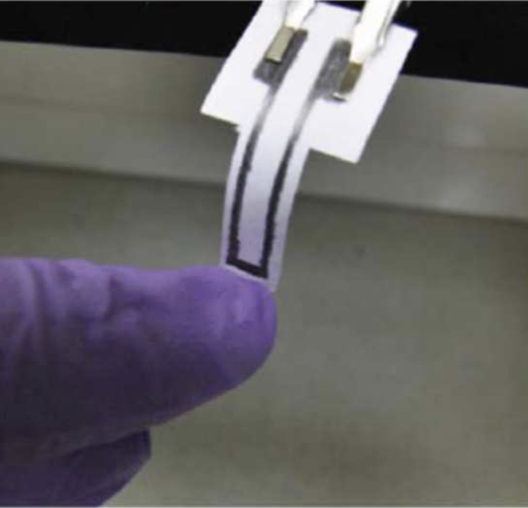
\includegraphics[width=0.7\textwidth,right]{flex-sensor.png}

\end{minipage}
\end{figure}




\section{Description}

The Graphite Strain Sensor is based on a conductive network of graphite particles deposited on a paper substrate.

When a pencil trace is drawn on paper, graphite particles adhere to the fibers, forming a thin conductive film.
 This film behaves as a disordered granular system where electrical conduction occurs through contacts between graphite particles.

Mechanical deformation affects this network:
\begin{itemize}
    \item Under tensile strain, the distance between particles increases, reducing electrical contacts and increasing resistance.
    \item Under compressive strain, particles are pushed closer together, improving connectivity and decreasing resistance.
\end{itemize}

The sensor response is therefore governed by variations in the percolation network and tunneling effects between neighboring particles.

Due to its structure, the sensor is highly sensitive to small deformations but also influenced by fabrication parameters such as graphite density,
 pencil grade, and environmental conditions (humidity, temperature).

The resulting resistance variation can be measured using a transimpedance circuit, to obtain a usable analog signal.

\section{Technical specification}

\centering
\begin{tabular}{lcccc}
\toprule
Parameter & Min & Typical & Max & Unit \\
\midrule
Supply voltage & -- & 5 & - & V \\
Output voltage & 0 & -- & 5 & V \\
Output current & -- & $10^{-7}$ & -- & A \\
Operating temperature & 10 & 20 & 35 & °C \\
Storage temperature & 0 & -- & 60 & °C \\
Humidity (operating) & 0 & 30 & 60 & \% \\
Sensor resistance & $10^5$ & $10^6$ & $10^7$ & $\Omega$ \\
Thickness & 15& -- & 35 & mm \\
Weight & 70 & -- & 140 & mg \\
Number of pins & \multicolumn{3}{c}{2} & -- \\
\bottomrule

\end{tabular}
\begin{tabular}{lcccc}
\toprule
Pad & name & Value &\\
\midrule
Pad 1 & Vin & VCC  \\
Pad 2 & Out  & Analog output \\
\bottomrule
\end{tabular}

\raggedright



\section{Pin Configuration}

\begin{center}
\begin{tabular}{lll}
\toprule
Pin Arduino & Signal & Description \\
\midrule
5V & VCC & Power supply to sensor and circuit \\
GND & GND & Common ground \\

A0 & AO & Amplified analog output \\
A1 & FLEX & Flex sensor input \\

D8 & CS & Digital Potentiometer \\
D11 & MOSI & Digital Potentiometer  \\
D13 & SCK &  Clock \\

A4 & SDA & I2C Data (OLED display) \\
A5 & SCL & I2C Clock (OLED display) \\

D2 & CLK & Encoder clock signal \\
D4 & DATA & Encoder data signal \\
D5 & SW & Encoder push button \\

D10 & TX & Bluetooth transmission \\
D9 & RX & Bluetooth reception \\


\bottomrule
\end{tabular}
\end{center}



\section{Kicad (Scheme and  PCB)}
\begin{figure}[h]
    \centering
    \begin{minipage}{0.48\textwidth}
        \centering
        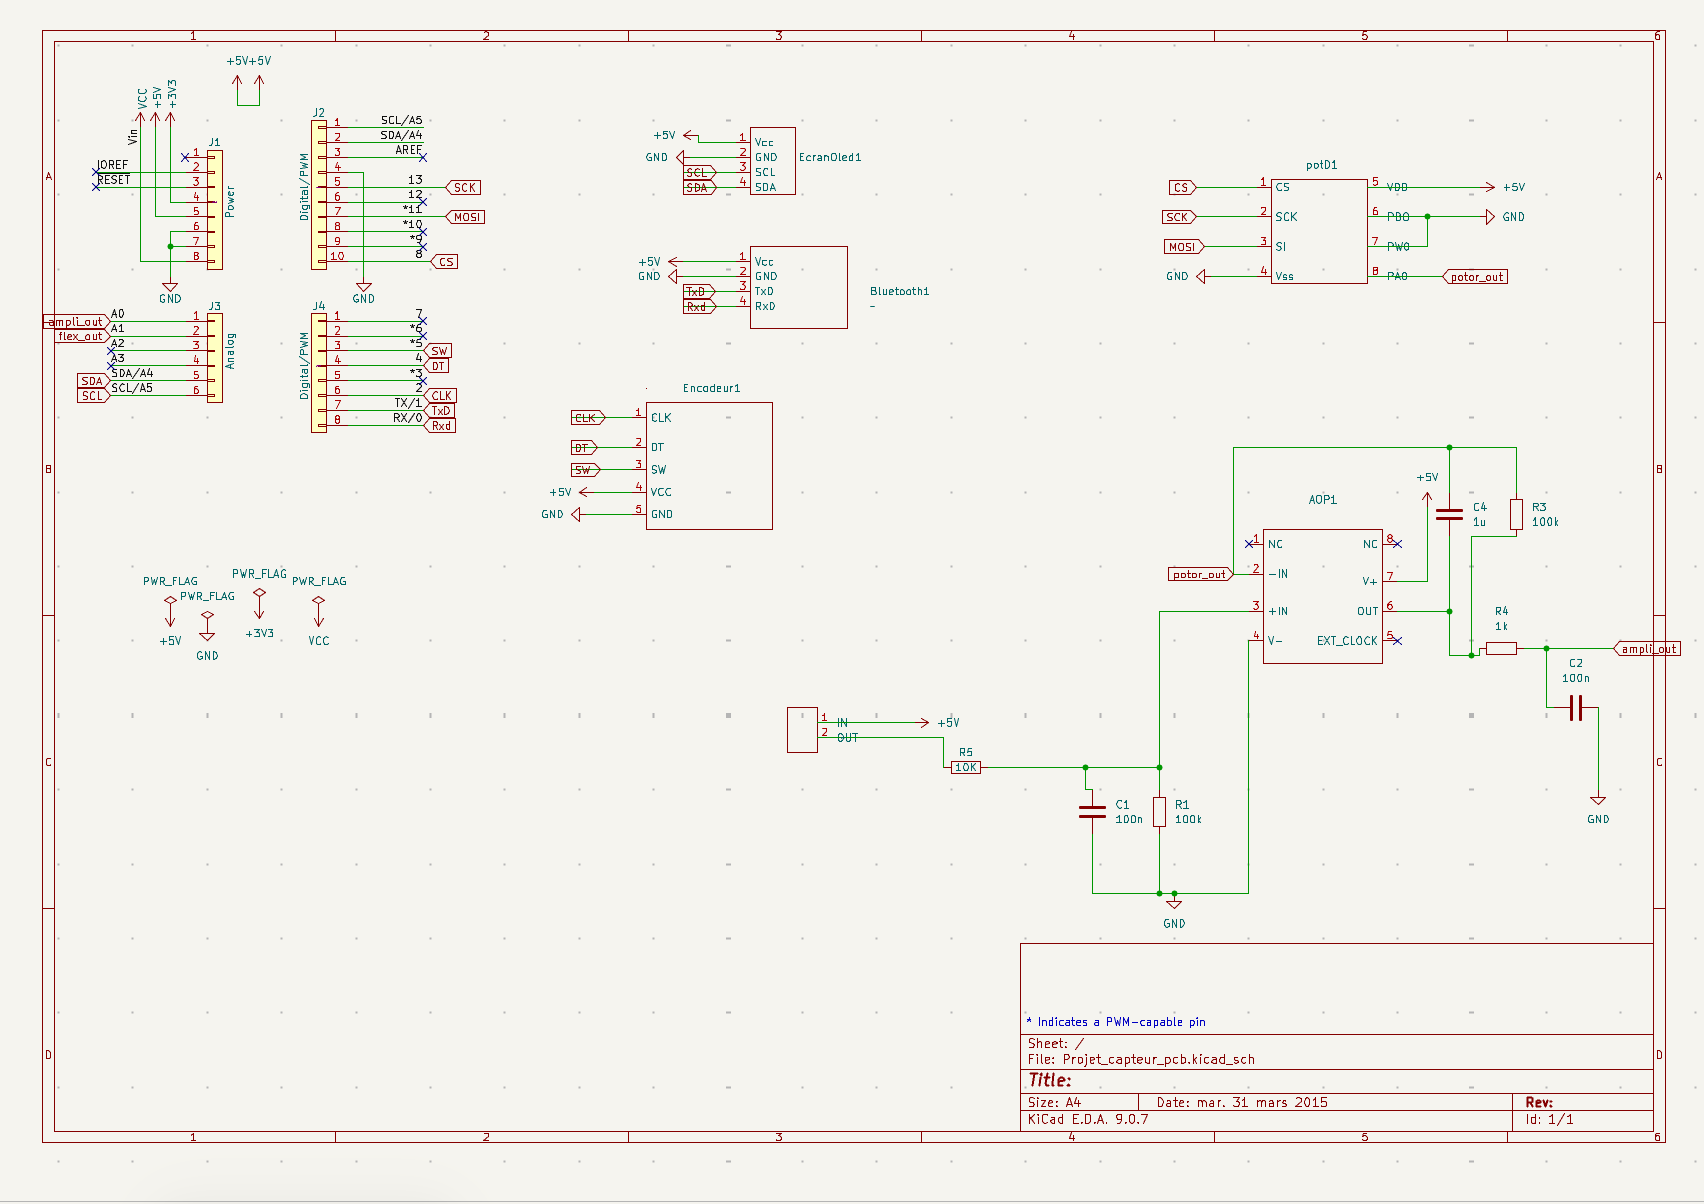
\includegraphics[width=\textwidth]{shm.png}
        \caption{Electrical diagram}
    \end{minipage}
    \hfill
    \begin{minipage}{0.48\textwidth}
        \centering
        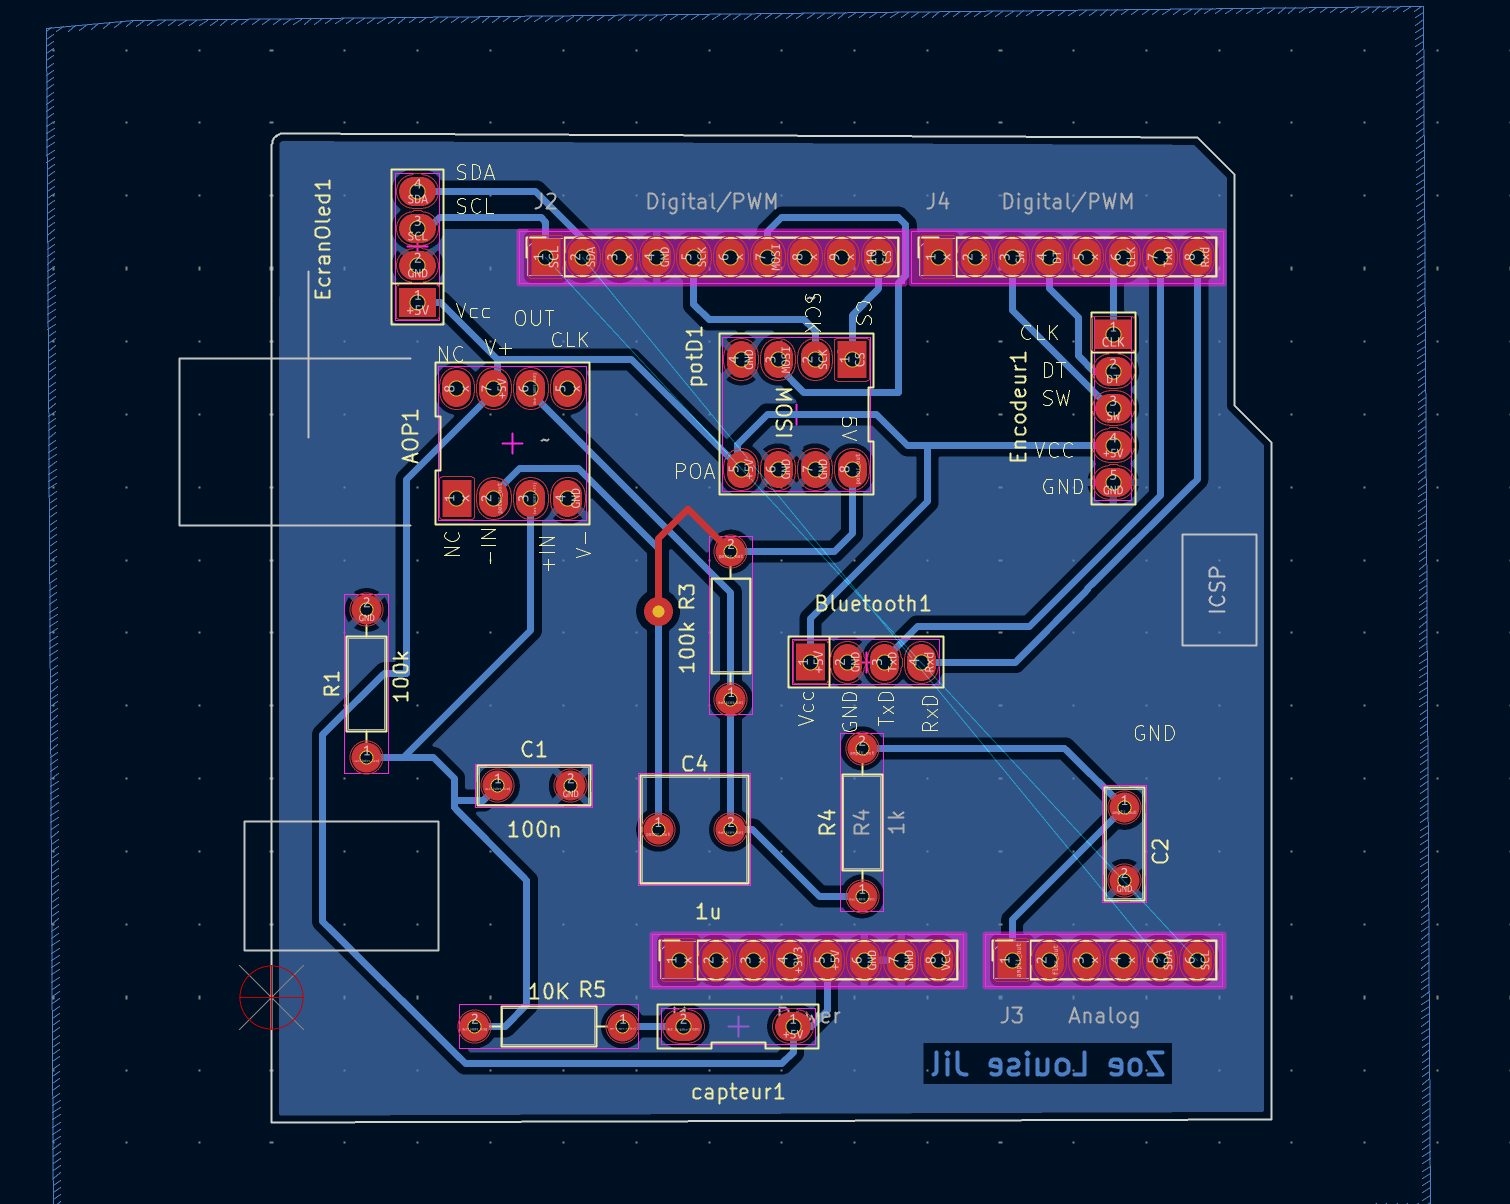
\includegraphics[width=\textwidth]{pcb.png}
        \caption{PCB routing}
    \end{minipage}
\end{figure}


\section{Low tech Captor}
\begin{center}
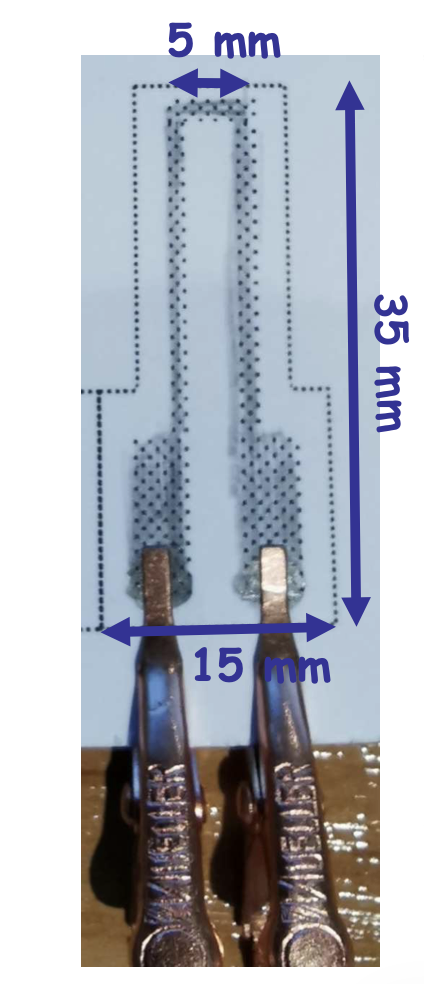
\includegraphics[width=0.3\textwidth, angle=90]{mesure.png}
\end{center}

\section{Typical Value}

\centering
\begin{tabular}{lc}
\toprule
Pencil Grade & Flat Resistance \\
\midrule
2B & \SI{1.93e6}{\ohm} \\
HB & \SI{4.08e6}{\ohm} \\
4B & \SI{5.69e5}{\ohm} \\
B  & \SI{1.80e6}{\ohm} \\
\bottomrule
\end{tabular}

\raggedright
\begin{figure}[h]
\centering

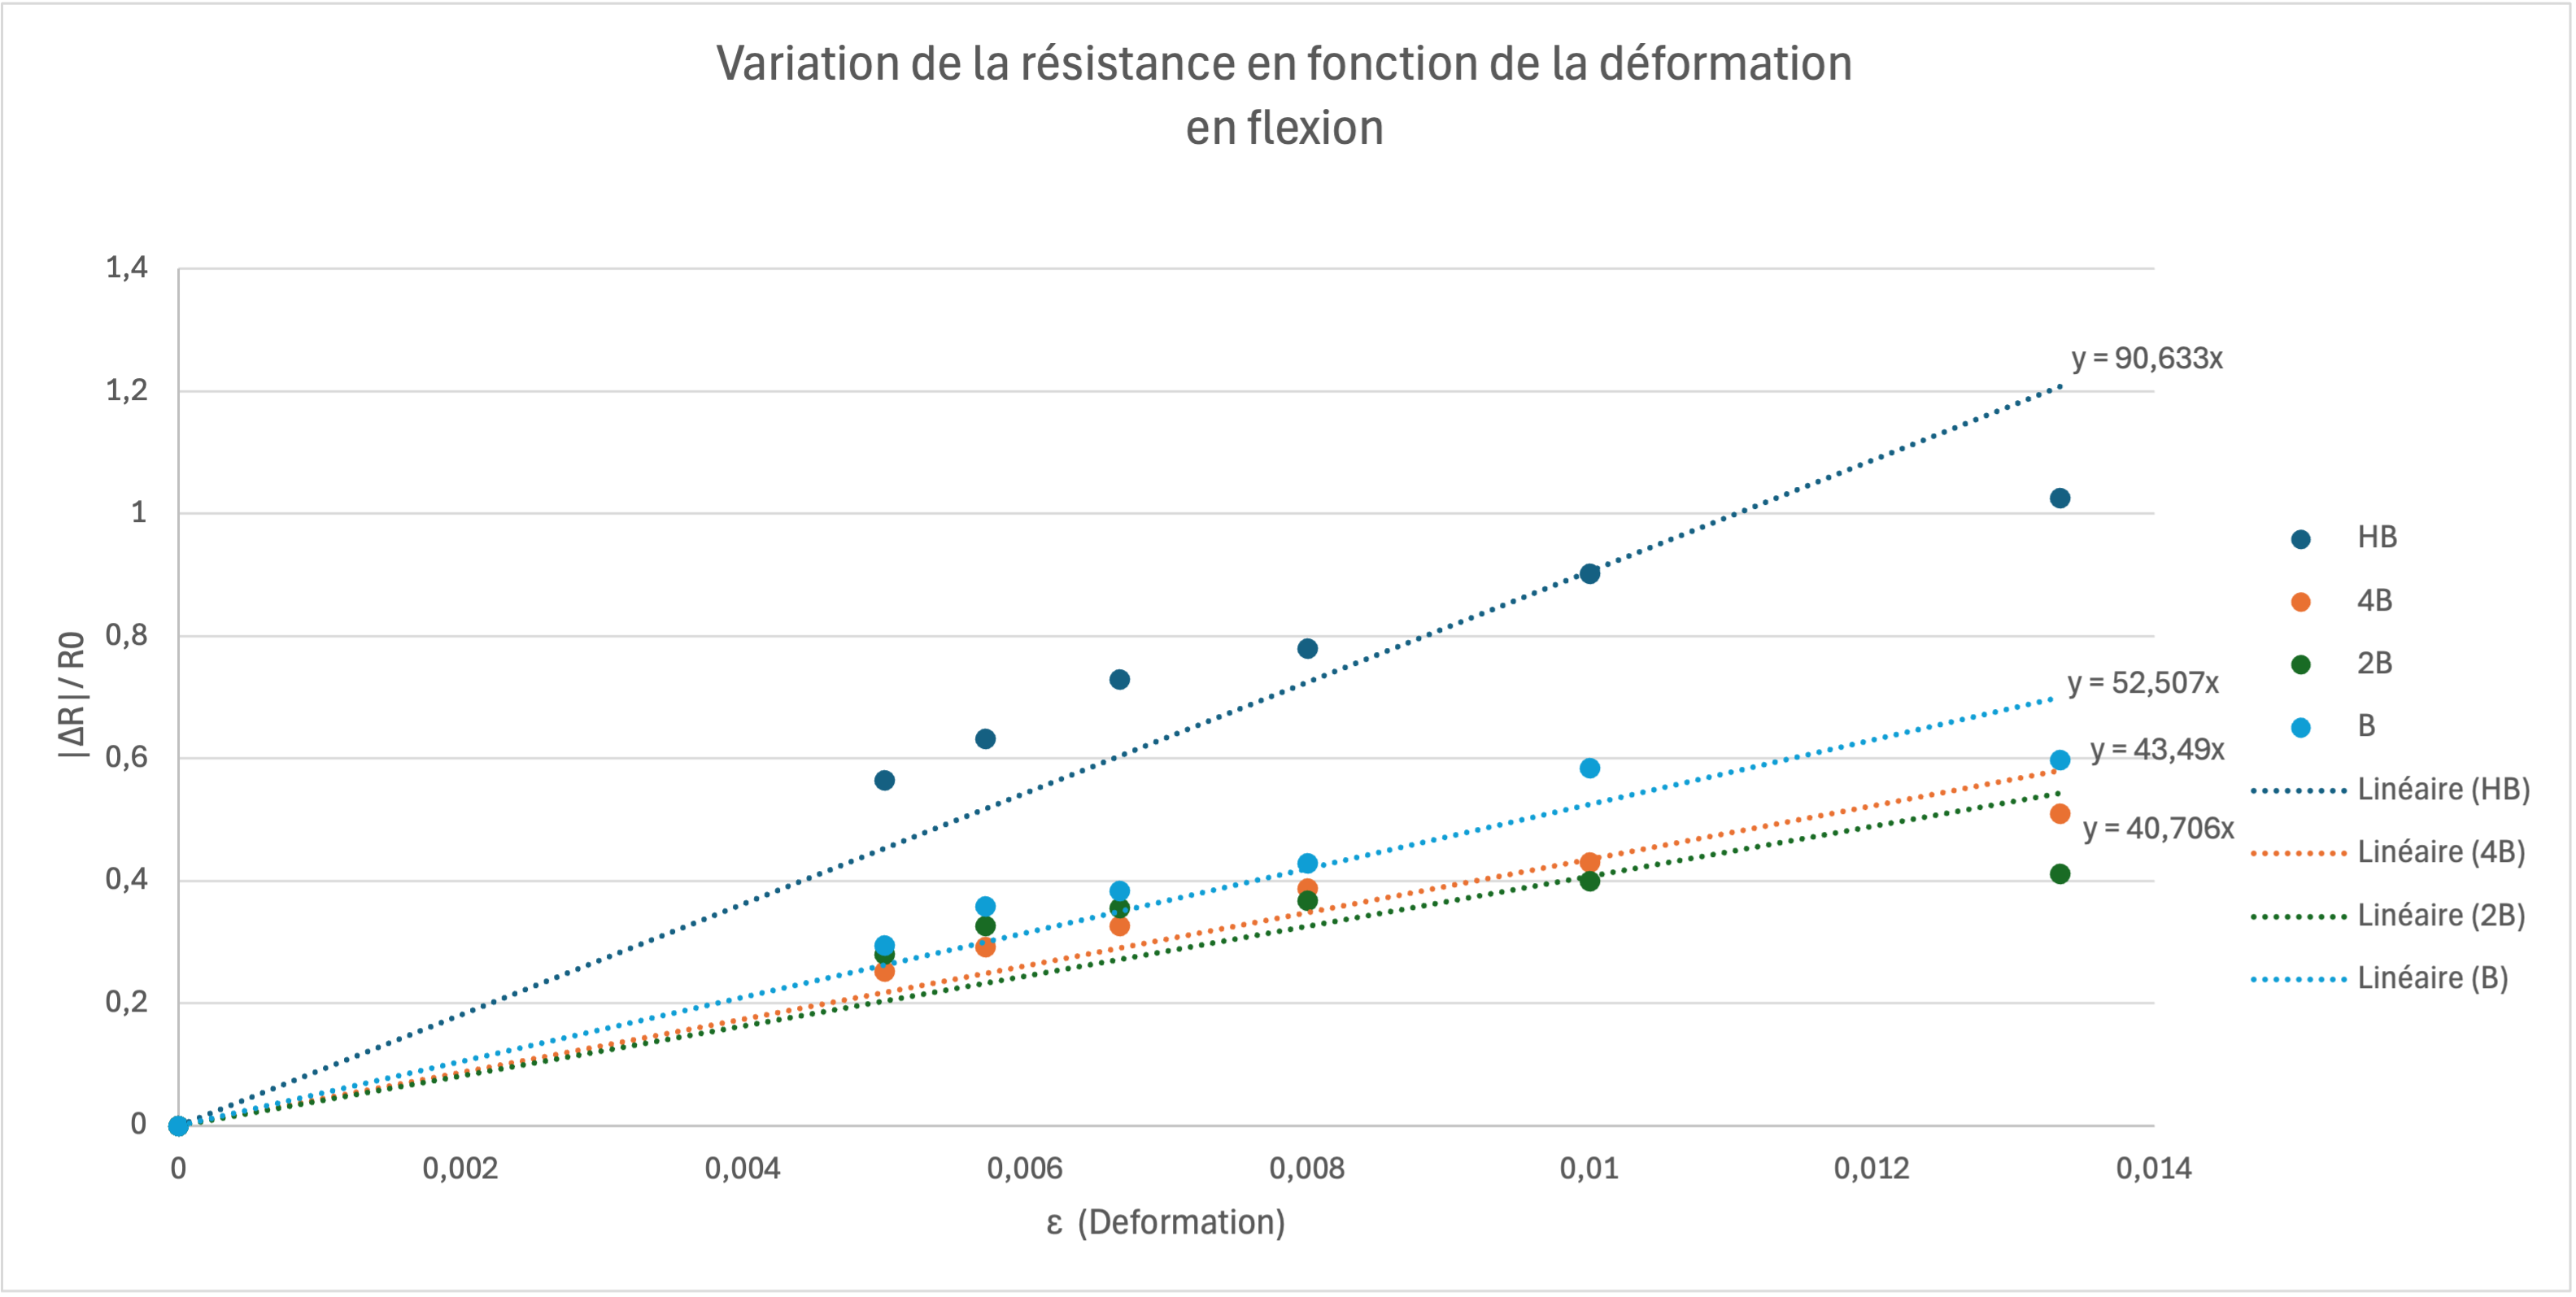
\includegraphics[width=0.9\textwidth]{resultat_flexion.png}
\caption{Bending result}

\vspace{0.5cm}

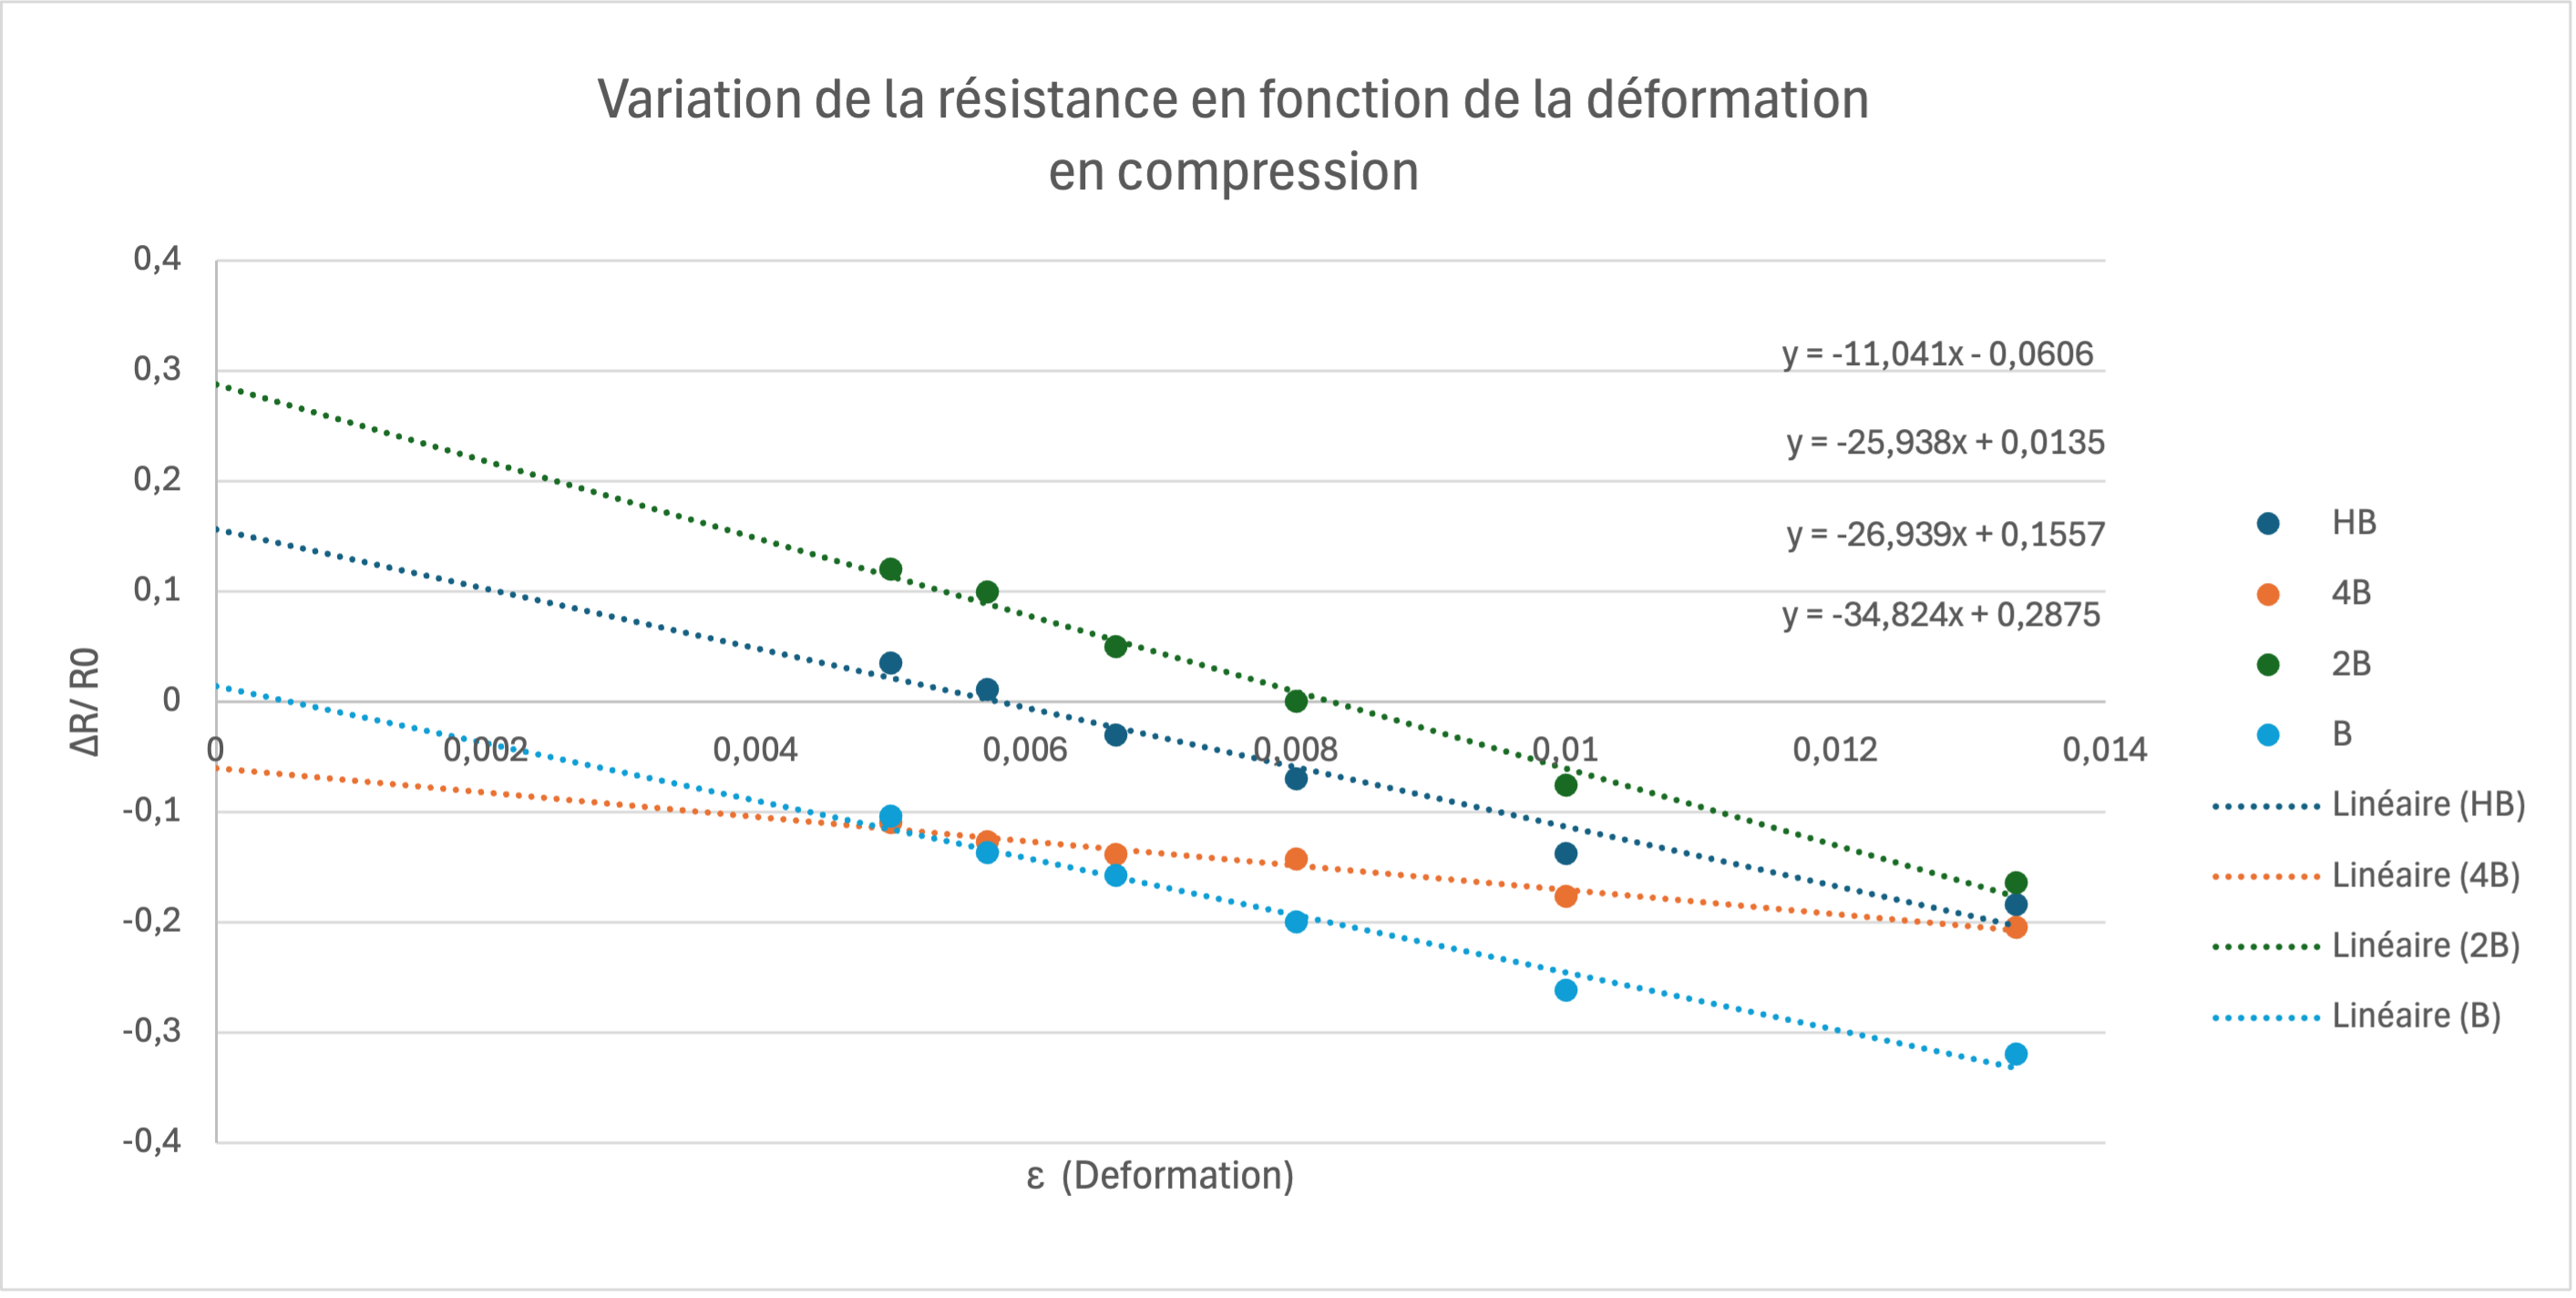
\includegraphics[width=0.9\textwidth]{Résultat_compression.png}
\caption{Compression result}

\end{figure}
\end{document}


